\chapter{Trusted Execution Environments (TEEs)}\label{chapter:tee}

Trusted Execution Environments do have a great potential for achieving a new
security level of mobile devices. In \parencite{mobile_tee}, an introduction
to TEEs for the mobile domain is given and will be recapped at this point.
TEEs do offer a parallel execution environment for applications including storage. A crucial part is the isolation of the TEE to its common counterpart, often called the Rich Execution Environment (REE) running on top of its underlying Rich OS (Android, Windows OS, Symbian OS). The main goal is to outsource sensitive operations from the REE to the TEE so that sensitive data won't leave
the secure world and to prevent malicious code from the Rich OS to interfere with this secure part. Security applications often make usage of tokens (hardware 
and software based, one-time tokens and two-factor authentication).
TEEs do have the potential of replacing them also with an increase of usability
for users.
Today, even every smartphone includes a TEE. Since ARM CPUs are quite popular in mobile devices, it is likely to find an ARM TrustZone TEE but there also do exist implementations for Intel (TXT) and AMD (Secure Execution Environment) that do behave quite similar.
A general TEE overview is shown in \autoref{fig:tee_structure} taken from the
official ARM website. TEEs can therefore be seen as a direct copy of the common
system, meaning that it has for instance also its own Thread and Handler modes.
\begin{figure}[htb]
  \centering
  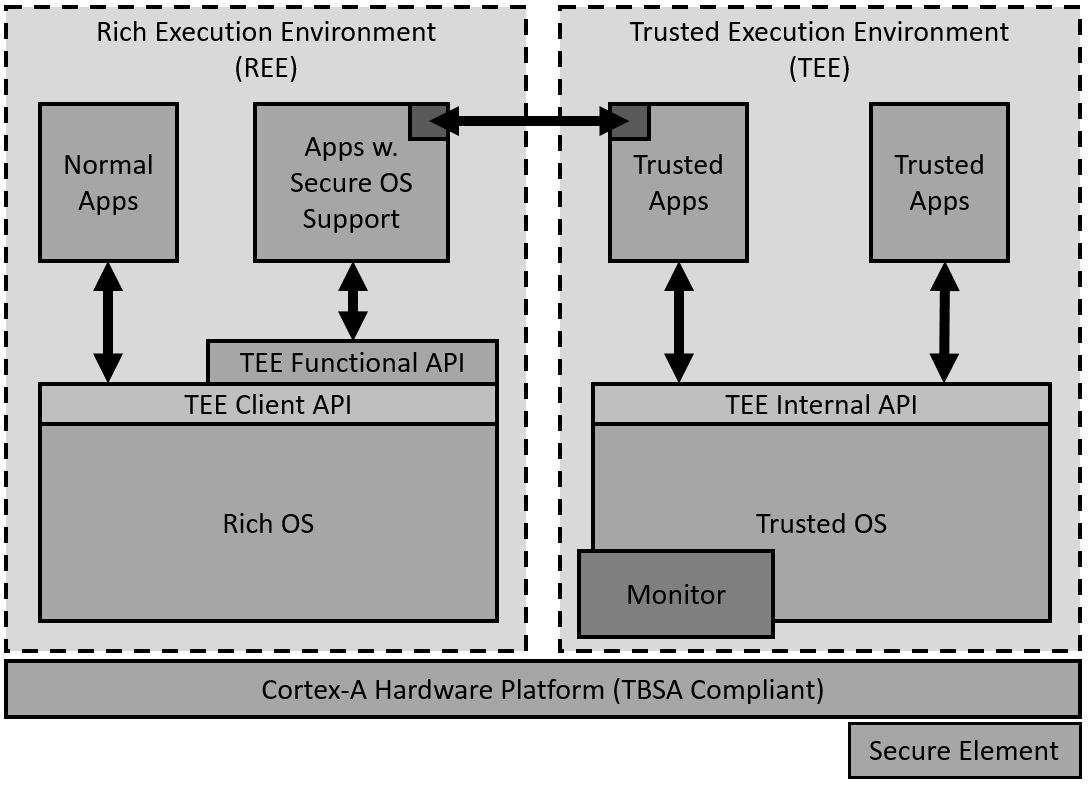
\includegraphics[scale=0.6]{figures/TEE_structure}
  \caption[General TEE Structure]{General TEE Structure taken from \parencite{tee_dev}}
  \label{fig:tee_structure}
\end{figure}
There do exist two main TrustZone technology concepts - the ARM TrustZone Technology for Cortex-A and Cortex-M Processors as well as the ARM TrustZone CryptoCell \parencite{trustzone}. Like mentioned before, the main concept of TEEs is the two seperated worlds, for instance by choosing an own physical CPU for each of them. A switch between them can be applied by a secure monitor (application processor) or by hardware (microcontrollers). The seperation however must not stop with CPU seperation but can also be applied to memory and 
software itself. The CryptoCell expands the security possibilities by providing
hardware support for security acceleration. It does include more efficient 
cryptographic engines, secure boot options as well as a root of trust element including key management. It acts as a complete seperate functional block to a CPU. Let's summarize the buzzwords like proposed in \parencite{tee_guide}:

\begin{itemize}
\item \textbf{Rich OS} is the common environment/operating system of a mobile device which focusses on applications and functionality but with a secondary concern for security matters. It is therefore open for third party applications
that can be downloaded by the user.
\item \textbf{TEE} is built on top of the Rich OS and offers a trusted environment using software but most importantly also hardware to achieve that goal. Only trusted applications are allowed to execute code inside of that environment. Is is designed to overcome software attacks out of the Rich OS.
\item \textbf{Secure Element (SE)} is a piece of hardware that is tamper-resistant within secure applications and secure data can be stored. It has very limited functionality while offering a high level of security. 
\end{itemize}

Some relations of using those technologies and their trade offs are shown in \autoref{fig:rich_os_tee_se}.
\begin{figure}[htb]
  \centering
  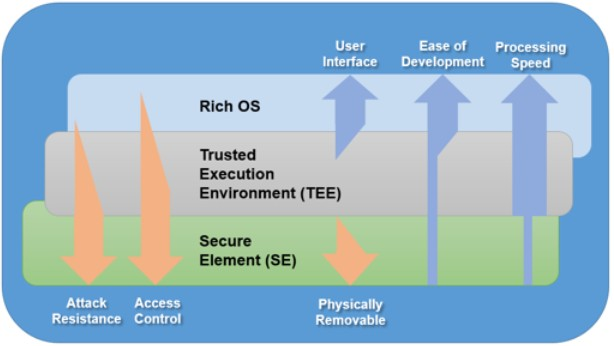
\includegraphics[scale=0.6]{figures/rich_os_tee_se}
  \caption[Rich OS, TEE and SE Comparison]{Rich OS, TEE and SE Comparison taken from \parencite{tee_guide}}
  \label{fig:rich_os_tee_se}
\end{figure}



%\begin{itemize}
%\item Secure Storage that really is not accessible from Rich OS
%\item Licensing mechanisms that can not be compromised
%\item Trusted User Interface
%\item mCommerce and mPayments
%\item BYOD - bring your own device -> handle confidential data at a secure place
%\end{itemize}


